
\documentclass[10pt,journal,compsoc, draftclsnofoot,onecolumn]{IEEEtran}
\usepackage{graphicx}
\ifCLASSOPTIONcompsoc

  \usepackage[nocompress]{cite}
\else
  % normal IEEE
  \usepackage{cite}
\fi

\ifCLASSINFOpdf

\else

\fi

\newcommand\MYhyperrefoptions{bookmarks=true,bookmarksnumbered=true,
pdfpagemode={UseOutlines},plainpages=false,pdfpagelabels=true,
colorlinks=true,linkcolor={black},citecolor={black},urlcolor={black},
pdftitle={Surviving the Big One},%<!CHANGE!
pdfsubject={Typesetting},%<!CHANGE!
pdfauthor={Michael D. Shell},%<!CHANGE!
pdfkeywords={Computer Society, IEEEtran, journal, LaTeX, paper,
             template}}%<^!CHANGE!




% correct bad hyphenation here
\hyphenation{op-tical net-works semi-conduc-tor}


\begin{document}

\title{Requirements\\ 3D object pose tracking for Robotics Grasping\\ Lux Vision \\ CS461 Fall 2017}


\author{Connor Campbell, Chase McWhirt, Jiawei Mo}
% \IEEEcompsocitemizethanks{\IEEEcompsocthanksitem holder\protect\\
% \IEEEcompsocthanksitem J. Doe and J. Doe are with Anonymous University.}% <-this % stops a space
% \thanks{Manuscript received April 19, 2005; revised August 26, 2015.}}

% \markboth{Journal of \LaTeX\ Class Files,~Vol.~14, No.~8, August~2015}%
% {Shell \MakeLowercase{\textit{et al.}}: Bare Advanced Demo of IEEEtran.cls for IEEE Computer Society Journals}

\IEEEtitleabstractindextext{%
\begin{abstract}
As robots and artificial intelligence become increasingly important in the modern age, they will need to be able to interact with their environment on their own, and computer vision is an integral part of a robot's understanding of its surroundings. Oregon State University's robotics department has an ongoing project attempting to improve computer vision, and this Capstone project is aimed at furthering that goal. Specifically, using machine learning to help a computer make appropriate adjustments to its calculations based on changes in lighting.
\end{abstract}

}


\maketitle

\IEEEdisplaynontitleabstractindextext
\IEEEpeerreviewmaketitle

\pagebreak
\tableofcontents
\pagebreak

\ifCLASSOPTIONcompsoc
\IEEEraisesectionheading{\section{Introduction}\label{sec:introduction}}
\else
\section{Introduction}
\label{sec:introduction}
\fi

\IEEEPARstart{}{}




\subsection{Purpose}
The purpose of this software will be to improve a computer's ability to identify a known object in an image in different lighting conditions.

\subsection{Scope}
The software will be able to determine the lighting conditions in a given image, then use that information to determine what parts of the image include the object it's looking for. Taking lighting conditions into account will allow the computer to be more selective when identifying pixels as part of the object it's looking for, which will reduce the number of false positives without losing accuracy. This will improve the computer's ability to interact with the environment with a robot arm.


\subsection{Overview}

\subsubsection{Product Perspective}
The object tracking system currently used by the University's robotics team has an issue with lighting. Shadows and different lighting intensities result in the objects the computer is looking for appearing as different colors. Currently, it accounts for this by identifying a large range of colors as potentially being part of the object. This, of course, results in a lot of false positives (pixels being labeled as part of the object when they actually aren't). This new approach will allow the computer to adjust the expected average for the specific lighting with a smaller acceptable range.

If the new programs prove to be more accurate than the ones currently in use, then the old identification system will be swapped out for the new one. As such, the differences in how the program interacts with the rest of the project should be minimal, to ensure a smooth transition.

\subsubsection{Product Functions}
The first function will determine the lighting diffuse and specular of the scene. It will be created using machine learning. In this case, the input will be an image (in the form of the color values of each pixel), and the outputs will be seven numbers that accurately describe the lighting of the scene.

The second function will then use the information provided by the first to identify which pixels in the image belong to the object. The larger project already has a means of determining an approximate mask of the image, so our function will use that along with the lighting information to generate a more precise mask. This may also utilize machine learning.

\subsubsection{User Characteristics}
These functions will primarily be used by the University's robotics research team. They won't be robust enough for complex, real world applications, but are rather meant to be a step forward for future research.


\subsubsection{Constraints}
This phase is a part of a big project. Our group is to undertake only the lighting changes during object grasping. As such, it will need to interact appropriately with the rest of the project. Since this program is meant to replace an older identification system, it will be ideal for the inputs and outputs to be similar, in order to minimize the need for adjustments to the rest of the project.


\subsection{Definitions}
\begin{itemize}
\item Pose tracking - The ability for a computer to determine the relative position of an object through computer vision.
%The pose tracking refers to robotic hand and object position changing that the computer is supposed to recognize the labels of hand, object and environment. 

\item OpenRave - An open source robot development platform, which can be used for robot motion planning. It reconstructs three dimensional scenes that allows developers to analyze robot movement. For instance, a different set of instructions is needed for a robot grabbing an object located above its hand as opposed to the side of the hand.

\item Surface Normal - The vector that is orthogonal to the surface. Another common vector is the Vertex Normal, which achieves more realistic light reflection than Surface Normal. However, for the purposes of this project, we will focus on the surface normal.

\item Diffuse - Accounts for the angle between the incoming light and the Surface Normal.

\item Specular - Accounts for the angle between the "perfect reflector" and the eye.

\item Machine learning -  An algorithm designed to take in example problems with the correct solutions generated by humans, in order to find patterns that humans may have trouble hard coding into the computer, until it eventually learns to solve the problems on its own.

\item Neural Network - A form of machine learning designed to mimic the activity of organic brains by simulating neurons firing in order. This can be simplified as a multiplying a series of matrices to the input.

\item Mask - in this context, a mask is a computer vision term that has to do with identifying objects in an image. A mask is a bitmap that labels each pixel in an image as either part of the object being identified or not.

\end{itemize}




\hfill
% \hfill August 26, 2015



\section{System Requirements}


\subsection{Functional requirements}
The end product will be two helper functions for the computer vision project.
The first will take an image of a scene and the initial position of the object being tracked as input and determine the diffuse and specular that describe the lighting of the scene.
These will be used to determine the color range that the computer should be looking for.
The second function will then use the images, diffuse, specular, and the approximate mask in order to determine a more accurate final mask.
The primary goal is to get these functions to properly track a robotic arm, and as a stretch goal is to attempt to do the same with a set of objects that the arm can manipulate.

Both of these functions will be made with machine learning.
They will be trained with a video of the arm moving around in such a way as to cast a shadow on itself, as well as in different lighting scenarios.
About one hundred and fifty key frames will be taken from the video for training and testing data.
The specular and diffuse will be measured by hand, as well as an accurate mask for the robotic arm using a image editing software, such as Photoshop.
The functions will be fed this data for it to train itself, and when it's done, it will be tested for accuracy.


\subsection{Performance requirements}
There are two primary performance requirements that we will be aiming for.
The first is for the final mask to label at least 95\% of the pixels in a given image correctly, as opposed to the 80\% accuracy of the method currently being used.
The second requirement is to reduce the size of the color range the computer is looking for.
The current method attempts to make up for variations in lighting and shade by using a large range of acceptable colors to be identified as the object.
Since the new method can account for the lighting on its own and adjust the expected average accordingly, we hope to reduce the range by a factor of ten, reducing the number of false positives, without losing a significant amount of true positives.

\section {Verification}
The accuracy of the functions is rather simple to verify. All need be done is for some of the example problems to be saved for testing purposes. Provide the inputs fr the examples to the functions and compare the output to the expected output. If a function answers some examples with sufficiently low accuracy, new examples similar to the ones it failed on can be generated specifically to train it for those scenarios.

  \section{Gantt Chart}
  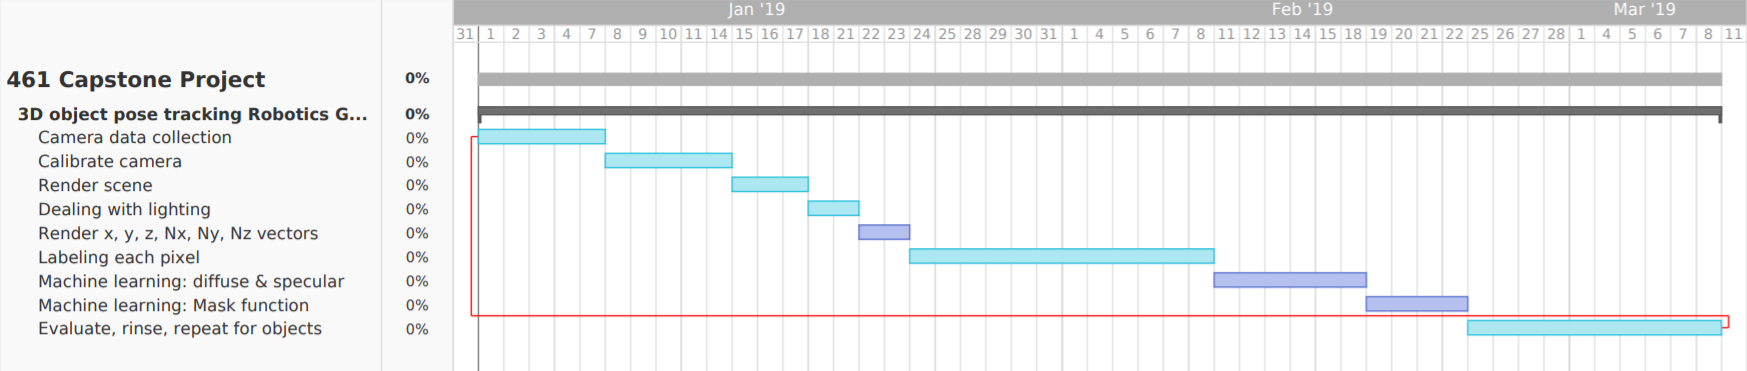
\includegraphics[width=\textwidth]{gantt.PNG}


\end{document}